\documentclass[12pt]{article}
\usepackage[english]{babel}
\usepackage{natbib}
\usepackage{url}
\usepackage[utf8x]{inputenc}
\usepackage{amsmath}
\usepackage{graphicx}
\graphicspath{{Images/}}
\usepackage{parskip}
\usepackage{fancyhdr}
\usepackage{vmargin}
\setmarginsrb{3 cm}{2.5 cm}{3 cm}{2.5 cm}{1 cm}{1.5 cm}{1 cm}{1.5 cm}

\title{Preparando datos con ayuda de Emacs}								% Title
\author{Martha Anahí Iñiguez Beltrán}						% Author
\date{\today}											% Date

\makeatletter
\let\thetitle\@title
\let\theauthor\@author
\let\thedate\@date
\makeatother

\pagestyle{fancy}
\fancyhf{}
\rhead{Física Computacional}
\lhead{\thetitle}
\cfoot{\thepage}

\begin{document}

\begin{titlepage}
\centering
    \vspace*{0.5 cm}
    
\includegraphics[width=5cm]{unison.jpg}\\[1.0 cm]	% University Logo
    \textsc{\LARGE Universidad de Sonora}\\[2.0 cm]	% University Name
    \textsc{\Large Departamento de ciencias exactas}\\[1.0 cm]
\textsc{\Large Física Computacional}\\[0.5 cm]
\rule{\linewidth}{0.2 mm} \\[0.4 cm]
{ \huge \bfseries \thetitle}\\
\rule{\linewidth}{0.2 mm} \\[1.5 cm]
\begin{minipage}{0.6\textwidth}
\begin{flushleft} \large
\emph{Alumno:}\\
\theauthor
\end{flushleft}
\end{minipage}~
\begin{minipage}{0.4\textwidth}
\begin{flushright} \large
214202804
\end{flushright}
\end{minipage}\\[2 cm]


{\large \thedate}\\[2 cm]

\vfill

\end{titlepage}

\tableofcontents
\pagebreak

\section{Introducción}

En esta actividad haremos uso intensivo del Editor Emacs para preparar los datos de sondeos de la Atmósfera descargados en la actividad anterior,  para su análisis posterior con Pandas. La preparación consta de limpieza y análisis de datos enfocados a las variables CAPE y PW.

La finalidad de la actividad 5 es el manejo de el editor de texto Emacs, así como reforzar el conocimiento de edición de scripts de shell. A continuación describiremos el significado físico de las variables CAPE y PW.

\section{Descripción de los conceptos físicos de CAPE y PW}

Dos conceptos importantes a abordar en ésta actividad son el CAPE y el PW, de los cuales se hizo un análisis de datos obtenidos de la estación de Narsarsuaq.

\textbf{CAPE}

Cuando hablamos de CAPE nos referimos a la energía potencial convectiva disponible (en ingles Convective Available Potential Energy).

En meteorología , la energía potencial convectiva disponible (CAPE), es la cantidad de energía que tendría una parcela de aire si se levantara una cierta distancia verticalmente a través de la atmósfera. CAPE es efectivamente la flotabilidad positiva de un paquete de aire y es un indicador de la inestabilidad atmosférica , lo que lo hace muy valioso para predecir el mal tiempo. Es una forma de inestabilidad de fluidos que se encuentra en atmósferas térmicamente estratificadas en las que un fluido más frío se superpone a uno más cálido. Como se explica a continuación, cuando una masa de aire es inestable, el elemento de la masa de aire que se desplaza hacia arriba se acelera por la diferencia de presión entre el aire desplazado y el aire ambiente a la altitud (más alta) a la que se desplazó. Esto generalmente crea nubes desarrolladas verticalmente por convección, debido al movimiento ascendente, que eventualmente puede conducir a tormentas eléctricas. También podría ser creado por otros fenómenos, como un frente frío. Incluso si el aire es más frío en la superficie, todavía hay aire más cálido en los niveles medios, que puede subir a los niveles superiores. Sin embargo, si no hay suficiente vapor de agua presente, no hay capacidad para la condensación, por lo tanto, no se formarán tormentas, nubes y lluvia.

\textbf{PW}

El PW (del ingles Precipitable Water) se refiere al agua precipitable.

El agua precipitable es la profundidad del agua en una columna de la atmósfera, si toda el agua en esa columna se precipitó como lluvia. Como profundidad, el agua precipitable se mide en milímetros o pulgadas. A menudo abreviado como "TPW" = total precipitable water.

\section{Limpieza y preparación de datos}

Para comenzar con la actividad se creó un script oara seleccionar la información de las variables CAPE y PW que se encuentran en el archivo de datos nombrado df2017-2.csv (creado en la actividad 4), esto usando el comando egrep y copiando la información a un nuevo archivo que nombraremos 2017-2CAPE\_PW.csv. Éste archivo se enviara al directorio de Actividad5.

\begin{verbatim}
#!/bin/bash
egrep '04270|CAPE|Precip' df2017-2.csv > df2017-2CAPE_PW.csv
\end{verbatim}
Editamos el archivo en EMACS para quitar los datos que no nos serán útiles. Los pasos a seguir fueron los siguientes:

\textbf{ctrl + spacebar:} Selecciona el texto a eliminar, desplazándonos con las flechas.

\textbf{ctr + w:} Elimina el texto seleccionado, pero se envía a la memoria temporal.

\textbf{ctrl + y:} Se trajo de vuelta el texto seleccionado.

\textbf{esc <:} Nos trasladamos al inicio del documento.

\textbf{esc + \%:} Es utilizado para remplazar una parte del
código por otra, cambiamos el texto guardado previamente en la memoria (ctrl + y) por una coma o espacios en blanco, dependiendo  lo que se quiera lograr.

\textbf{!:} Confirma los campos.

Al finalizar los pasos anteriores solo nos quedaron los datos que necesitamos acomodados por columnas: Lanzamiento, fecha, CAPE y PW en ese orden.

y por último se separan los datos en dos archivos, uno para cada lanzamiento (00Z y 12Z):

\begin{verbatim}
#!/bin/bash
egrep '00Z' df2017-2CAPE_PW.csv > df2017-2CAPE_PW_00Z.csv
egrep '12Z' df2017-2CAPE_PW.csv > df2017-2CAPE_PW_12Z.csv
\end{verbatim}

El anterior script selecciona los renglones que tienen 00Z y los envía al archivo df2017CAPE\_PW\_00Z.csv, y a los renglones con 12Z los envía al archivo df2017CAPE\_PW\_12Z.csv.

A cada uno de los archivos se le elimina el inicio del renglón pues todos los datos correponen al mismo lanzamiento: 00Z o 12Z.

\section{Análisis de datos}

A continuación se muestra el código en Python el cual se utilizó para hacer el análisis de datos.

\begin{verbatim}
import pandas as pd
import numpy as np
import matplotlib.pyplot as plt

df = pd.read_csv("df2017_capepw00Z.csv", header=None, names=['Date', 'CAPE', 'PW'])

df.CAPE=pd.to_numeric(df.CAPE, errors='coerce')
df.head()

df['Ndate'] = pd.to_datetime(df['Date'], format='%d %m %Y')
df['month'] = df['Ndate'].dt.month
df.head()

import seaborn as sns
import matplotlib.pyplot as plt
ax = sns.boxplot(x="month", y="CAPE", data=df)
plt.show()

import seaborn as sns
import matplotlib.pyplot as plt
ax = sns.boxplot(x="month", y="PW", data=df)
plt.show()

import seaborn as sns
sns.set(style="darkgrid", color_codes=True)

g = sns.jointplot("CAPE", "PW", data=df, kind="reg",
                   color="r", size=7)
plt.show(g)

g = sns.lmplot(x="CAPE", y="PW", hue="month",
               truncate=True, size=5, data=df)
plt.show(g)
\end{verbatim}

\pagebreak

\section{Resultados}

A continuación se muestran los resultados del análisis de datos.

\subsection{CAPE}

Se muestran los diagramas de la energía potencial convectiva disponible para cada uno de los lanzamientos (Figura 1 y 2):

\begin{figure}
\begin{centering}
  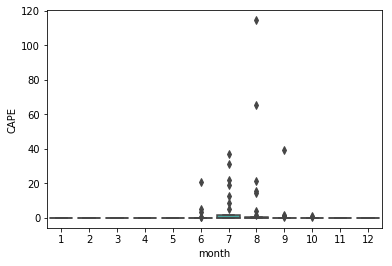
\includegraphics[scale = 0.8]{CAPE00Z.png}
  \caption{CAPE 00Z}
\end{centering}
\end{figure}

\begin{figure}
\begin{centering}
  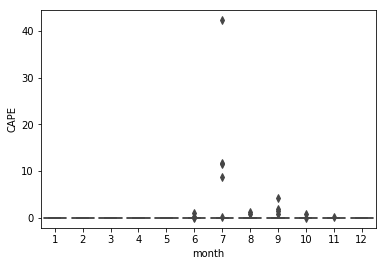
\includegraphics[scale = 0.8]{CAPE12Z.png}
  \caption{CAPE 12Z}
\end{centering}
\end{figure}

\subsection{PW}

A continuación se muestran los diagramas de cajas del agua precipitable para cada uno de los lanzamientos (Figura 3 y 4):

\begin{figure}
\begin{centering}
  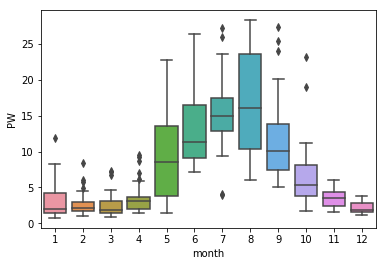
\includegraphics[scale = 0.8]{PW00Z.png}
  \caption{PW 00Z}
\end{centering}
\end{figure}

\begin{figure}
\begin{centering}
  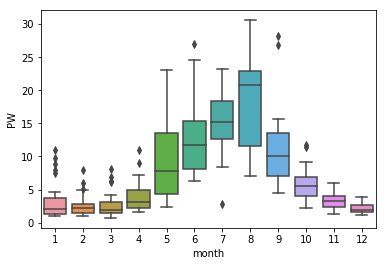
\includegraphics[scale = 0.8]{PW12Z.png}
  \caption{PW 12Z}
\end{centering}
\end{figure}

\subsection{Relación de PW y CAPE}

A continuación se muestran las gráficas de la relación entre el agua precipitable y la energía potencial convectiva disponible (Figura 5 y 6):

\begin{figure}
\begin{centering}
  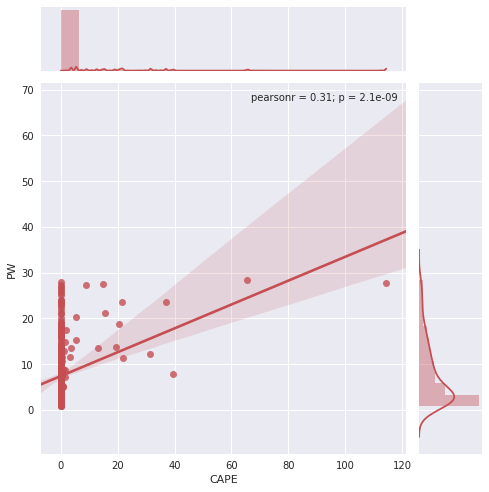
\includegraphics[scale = 0.8]{PW_CAPE00Z.png}
  \caption{Relación de PW y CAPE 00Z}
\end{centering}
\end{figure}

\begin{figure}
\begin{centering}
  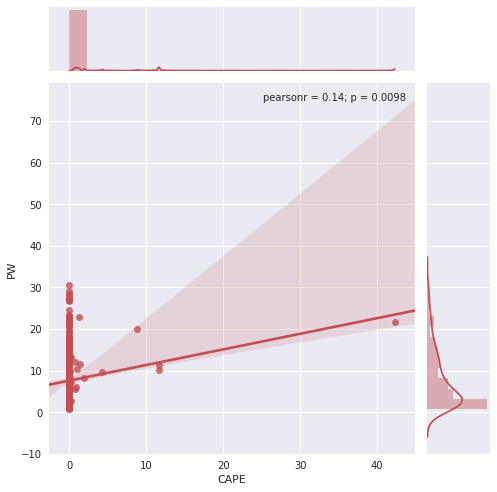
\includegraphics[scale = 0.8]{PW_CAPE12Z.png}
  \caption{Relación de PW y CAPE 12Z}
\end{centering}
\end{figure}

\subsection{Pareados}

A continuación se muestra las gráficas de los pareados, es decir, uno en función del otro pero de cada mes (Figura 7 y 8):

\begin{figure}
\begin{centering}
  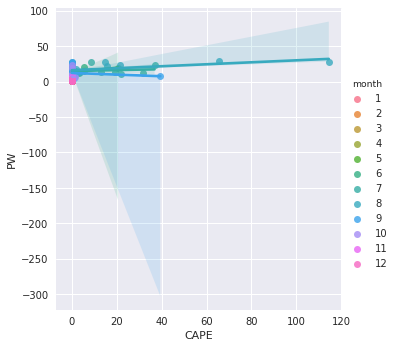
\includegraphics[scale = 0.8]{PW_CAPE200Z.png}
  \caption{Pareado 00Z}
\end{centering}
\end{figure}

\begin{figure}
\begin{centering}
  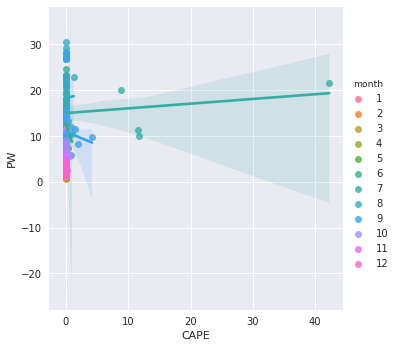
\includegraphics[scale = 0.8]{PW_CAPE212Z.png}
  \caption{Paread 12Z}
\end{centering}
\end{figure}

\section{Conclusión}

Como conclusión podemos añadir que usamos lo que sabíamos del uso del lenguaje de programación Python junto con el manejo de scripts de shell, lo que nos llevó a realizar una actividad más compleja y completa, juntando el conocimiento adquirido de las actividades anteriores y ahora, aprendimos nuevas maneras de graficar con la biblioteca seaborn.

\section{Bibliografía}

-Convective Available Potential Energy (2018) De Wikipedia.org. Recopilado el 06 de mars¿zo del 2018: https://en.wikipedia.org/wiki/Convective\_available\_potential\_energy

-Precipitable Water (2018) de Wikipedia.org. Recopilado el 06 de marzo del 2018: https://en.wikipedia.org/wiki/Precipitable\_water

--Atmospheric Soundings (2018) College o Engineering, University of Wyoming. Recuperado el 03 de marzo del 2018: $http://weather.uwyo.edu/upperair/sounding.html$

\section{Apéndice}

A continuación se responden algunas preguntas acerca de la actividad.

\textbf{¿Cómo se te hizo esta actividad? ¿Compleja, Difícil, Sencilla?}

Me pareció compleja pero completa.

\textbf{¿Qué te llamó más la atención?}

Me llamó la atención la manera de graficar datos estadísticos con seaborn.

\textbf{¿Qué parte fue la que menos te interesó hacer?}

Toda la actividad me pareció interesante.

\textbf{¿Cómo mejorarías esta actividad? ¿Qué le faltó? ¿Qué sobró?}

La actividad así está bien.

\textbf{¿Hasta este punto, que te parece el uso de Jupyter para programar en Python? }

Es muy completo y sencillo.

\end{document}
